\documentclass[a4paper,12pt]{article}
\usepackage{graphicx}
\usepackage{geometry}
\usepackage{fancyhdr}
\usepackage{float}
\usepackage[colorlinks=true, linkcolor=blue, citecolor=blue, urlcolor=blue]{hyperref}
\geometry{a4paper, margin=1in}

% Configure the header using fancyhdr
\pagestyle{fancy}
\fancyhf{} % Clear all header and footer fields
\fancyhead[L]{28.11.2024} % Left-aligned header
\fancyhead[C]{MADE Data Report --- Asheer Ali (22993810)} % Center-aligned header
\fancyhead[R]{\thepage} % Right-aligned header (page number)
\renewcommand{\headrulewidth}{0.4pt} % Line under header

% Title configuration
\title{Traffic Crash Patterns: Assessing the Influence of Human Factors}
\author{} % Remove author to suppress it
\date{} % Empty date to suppress it

\begin{document}

% Custom title block
\begin{center}
    \textbf{\Large Traffic Crash Patterns: Assessing the Influence of Human Factors} \\[1em]
    Asheer Ali \hspace{2cm} 28.11.2024
\end{center}

\section{Questions}
\begin{itemize}
    \item How do driver characteristics (e.g., age, sex, use of safety equipment) correlate with injury severity in crashes?
    \item What are the most common vehicle types and conditions associated with high-severity crashes?
\end{itemize}

\section{Data Sources}
\subsection{Descriptions of Data Sources}
\begin{itemize}
    \item \textbf{Traffic Crashes - People:} This dataset contains details of individuals involved in traffic incidents, including demographics, safety equipment use, and injury severity \cite{traffic_crashes_people}.
    
    \begin{figure}[H]
        \centering
        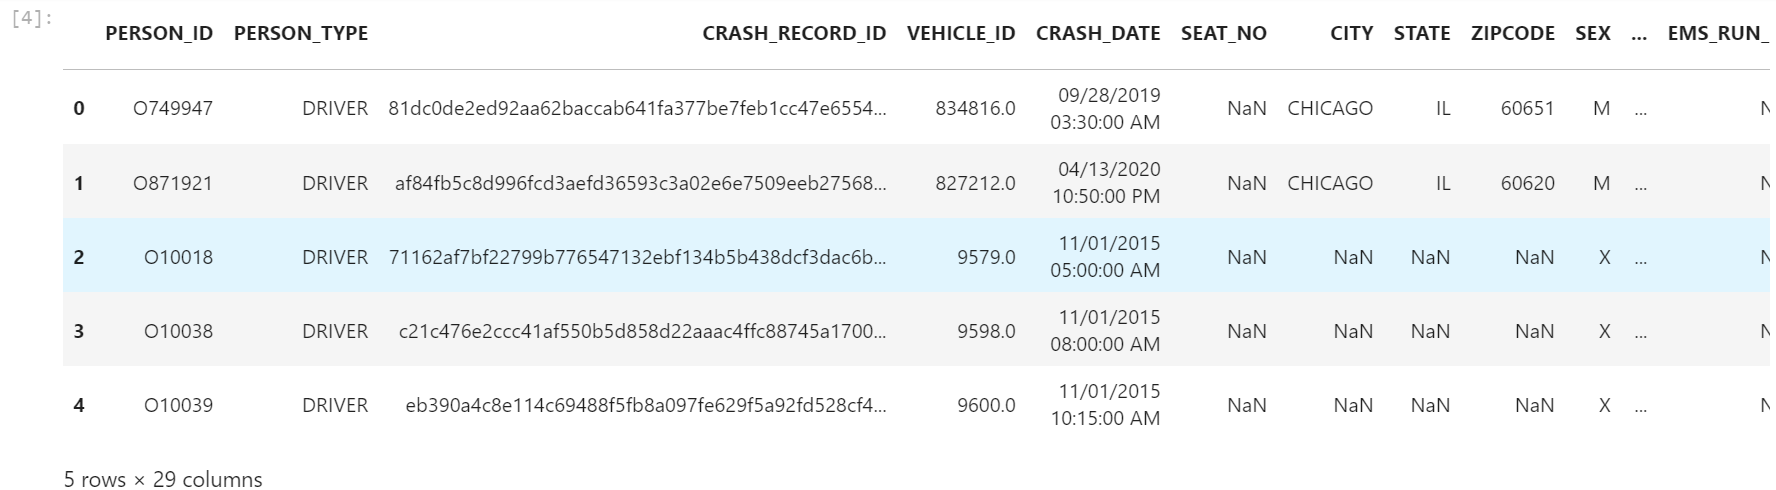
\includegraphics[width=1\linewidth]{images/dataset1.png}
        \caption{First 5 rows of traffic crashes people dataset}
        \label{fig:people}
    \end{figure}
    
    \item \textbf{Traffic Crashes - Vehicles:} Provides records of vehicles involved in crashes, including type, direction, and damage details \cite{traffic_crashes_vehicles}.
    
    \begin{figure}[H]
        \centering
        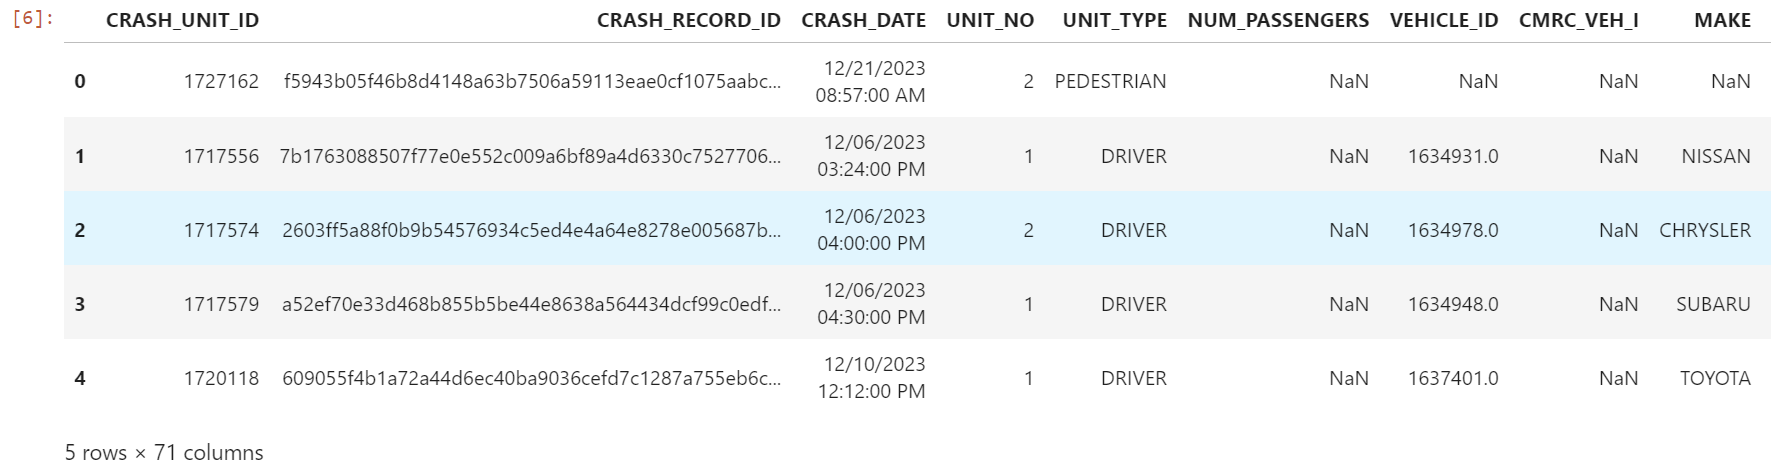
\includegraphics[width=1\linewidth]{images/dataset2.png}
        \caption{First 5 rows of traffic crashes vehicle dataset}
        \label{fig:vehicles}
    \end{figure}
\end{itemize}

\subsection{Structure and Quality of Data Sources}
\begin{itemize}
    \item \textbf{People Dataset:} Contains individual-level data with fields for demographics, safety equipment use, and injury severity. Missing values exist but can be handled through removing the rows with Nan values, as the nan values are not present that much in the selected columns. \cite{github_repo}.
    \item \textbf{Vehicle Dataset:} Vehicle-level data with fields for type, damage, and direction. Data quality is high, with minimal missing values.
\end{itemize}

\subsection{Licenses and Permissions}
Both datasets are publicly available under open-data licenses, allowing use with proper attribution \cite{traffic_crashes_people, traffic_crashes_vehicles}.

\section{Data Pipeline}
The data pipeline is implemented using Python and consists of the following steps:
\begin{itemize}
    \item \textbf{Extractor:} Downloads CSV files from the given URLs.
    \item \textbf{Transformer:} Processes the data with:
        \begin{itemize}
            \item Removing unnecessary columns.
            \item Handling missing values through imputation.
            \item Standardizing date formats for consistency.
        \end{itemize}
    \item \textbf{Loader:} Stores the cleaned datasets in an SQLite database for efficient access.
\end{itemize}

\begin{figure}
    \centering
    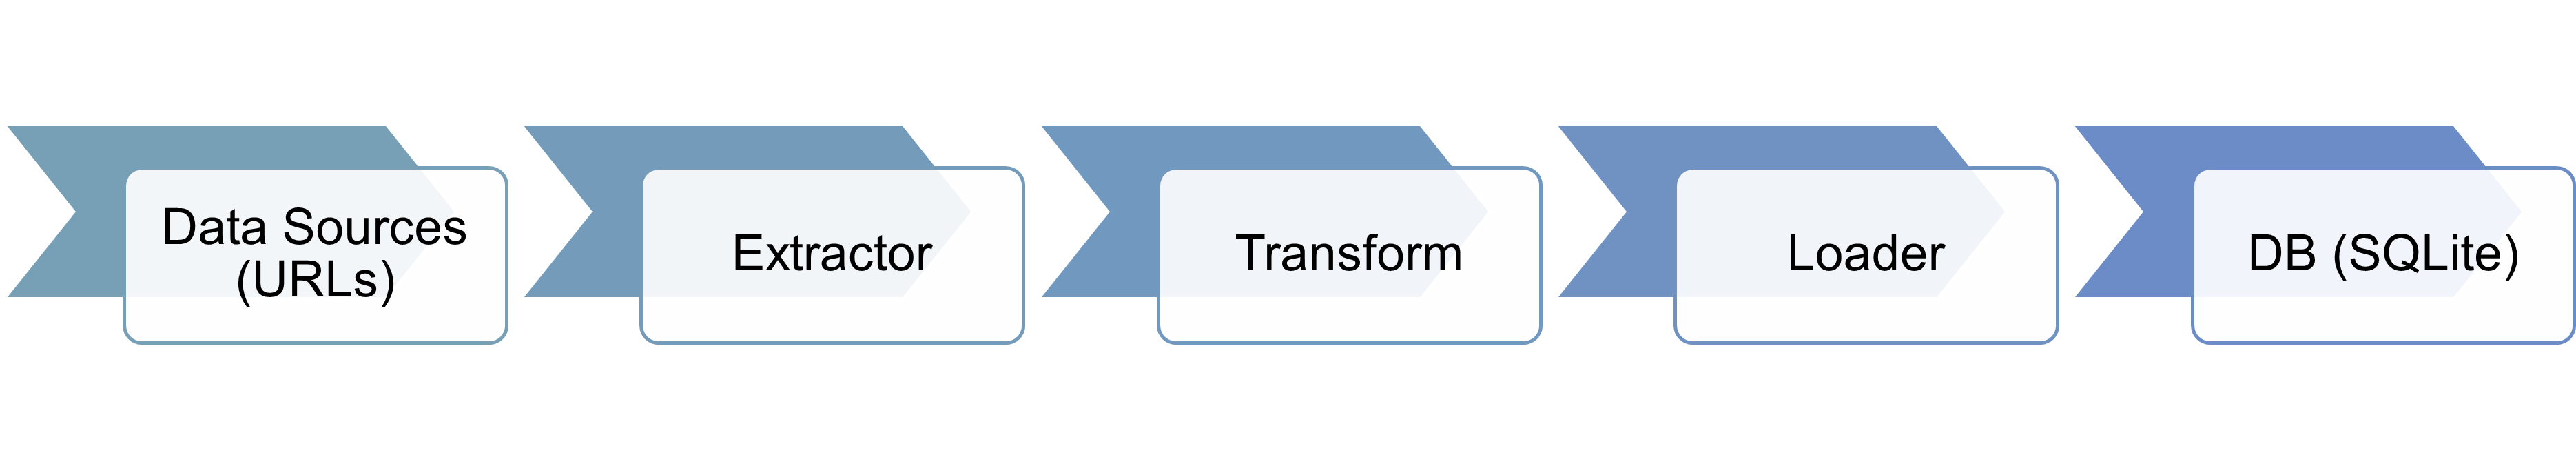
\includegraphics[width=1\linewidth]{images/Picture1.png}
    \caption{ETL Pipeline}
    \label{fig:ETL-pipeline}
\end{figure}

\section{Results and Limitations}
\subsection{Results}
\begin{itemize}
    \item Cleaned datasets stored in SQLite database.
    \item Data ready for analysis to address project questions about injury severity and crash patterns.
\end{itemize}

\subsection{Limitations}
\begin{itemize}
    \item Missing data for certain fields may impact analysis accuracy.

\end{itemize}

\section{References}
\bibliographystyle{plain}
\bibliography{reference}
\end{document}
